% Digital Logic Report Template
% Created: 2020-01-10, John Miller

%==========================================================
%=========== Document Setup  ==============================

% Formatting defined by class file
\documentclass[11pt]{article}

% ---- Document formatting ----
\usepackage[margin=1in]{geometry}	% Narrower margins
\usepackage{booktabs}				% Nice formatting of tables
\usepackage{graphicx}				% Ability to include graphics

%\setlength\parindent{0pt}	% Do not indent first line of paragraphs 
\usepackage[parfill]{parskip}		% Line space b/w paragraphs
%	parfill option prevents last line of pgrph from being fully justified

% Parskip package adds too much space around titles, fix with this
\RequirePackage{titlesec}
\titlespacing\section{0pt}{8pt plus 4pt minus 2pt}{3pt plus 2pt minus 2pt}
\titlespacing\subsection{0pt}{4pt plus 4pt minus 2pt}{-2pt plus 2pt minus 2pt}
\titlespacing\subsubsection{0pt}{2pt plus 4pt minus 2pt}{-6pt plus 2pt minus 2pt}

% ---- Hyperlinks ----
\usepackage[colorlinks=true,urlcolor=blue]{hyperref}	% For URL's. Automatically links internal references.

% ---- Code listings ----
\usepackage{listings} 					% Nice code layout and inclusion
\usepackage[usenames,dvipsnames]{xcolor}	% Colors (needs to be defined before using colors)

% Define custom colors for listings
\definecolor{listinggray}{gray}{0.98}		% Listings background color
\definecolor{rulegray}{gray}{0.7}			% Listings rule/frame color

% Style for Verilog
\lstdefinestyle{Verilog}{
	language=Verilog,					% Verilog
	backgroundcolor=\color{listinggray},	% light gray background
	rulecolor=\color{blue}, 			% blue frame lines
	frame=tb,							% lines above & below
	linewidth=\columnwidth, 			% set line width
	basicstyle=\small\ttfamily,	% basic font style that is used for the code	
	breaklines=true, 					% allow breaking across columns/pages
	tabsize=3,							% set tab size
	commentstyle=\color{gray},	% comments in italic 
	stringstyle=\upshape,				% strings are printed in normal font
	showspaces=false,					% don't underscore spaces
}

% How to use: \Verilog[listing_options]{file}
\newcommand{\Verilog}[2][]{%
	\lstinputlisting[style=Verilog,#1]{#2}
}




%======================================================
%=========== Body  ====================================
\begin{document}

\title{ELC 2137 Lab 5: Subtracting}
\author{CJ Jones, Ashlie Lackey}

\maketitle


\section*{Summary}

The purpose of this lab was to learn how to use the hardware description language Verilog to test digital circuits through designing and making testbenches. By coding a half-, full-, and 2-bit adder and testing them, skills in organizing files, learning syntax, and understanding gate-level code were obtained. This provides students with a basis for coding in Verilog, which will later be utilized for working with the FPGA Basys3 boards.


\section*{Q\&A}

\begin{enumerate}
	\item What is one thing that you still don’t understand about Verilog?
	
	We are still confused as how to properly run testbenches, and how to look for errors when the results don't look like how they are expected to.
\end{enumerate}




\section*{Results}

Below are the results for running the half-, full-, and 2-bit adders. The design and testbench code for each adder is included along with each expected results table and the block diagram of each digital circuit. As the ERT's and screenshots each indicate, the results from the testbench simulations do match what is expected.
\begin{figure}
	\includegraphics[width=1.0\textwidth]{"HalfAdderDia"}
	\caption{Block Diargram of the Half Adder}
\end{figure}
\clearpage

\begin{figure}[ht]\centering
	\begin{tabular}{l|rrrr}
		Time (ns): & 0 & 10 & 20 & 30 \\
		\midrule 
		a & 0 & 1 & 0 & 1 \\
		b & 0 & 0 & 1 & 1 \\
		\midrule
		c & 0 & 0 & 0 & 1 \\
		s & 0 & 1 & 1 & 0 \\ 
		\bottomrule
	\end{tabular}\medskip
	
	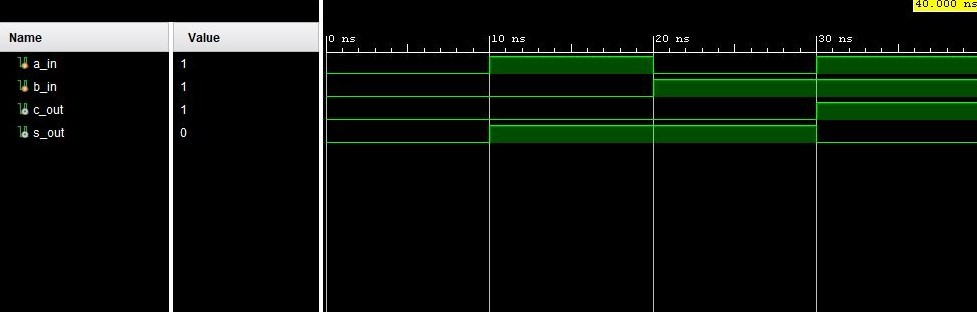
\includegraphics[width=1.0\textwidth]{HalfAdder}
	\caption{Half Adder simulation waveform and ERT}
	\label{fig:sim_with_table}
\end{figure}


\clearpage

\begin{figure}
	\includegraphics[width=1.0\textwidth]{"FullAdderDia"}
	\caption{Block Diagram of Full Adder}
\end{figure}
\clearpage

\begin{figure}[ht]\centering
	\begin{tabular}{l|rrrrrrrr}
		Time (ns): & 0 & 10 & 20 & 30 & 40 & 50 & 60 & 70 \\
		\midrule 
		a &  0 & 1 & 0 & 1 & 0 & 1 & 0 & 1 \\
		b & 0 & 0 & 1 & 1 & 0 & 0 & 1 & 1\\
		cin & 0 & 0 & 0 & 0 & 1 & 1 & 1 & 1 \\
		\midrule
		c & 0 & 0 & 0 & 1 & 0 & 1 & 1 & 1 \\
		s & 0 & 1 & 1 & 0 & 1 & 0 & 0 & 1 \\ \bottomrule
	\end{tabular}\medskip
	
	\includegraphics[width=1.0\textwidth]{FullAdder}
	\caption{Full Adder simulation waveform and ERT}
	\label{fig:sim_with_table}
\end{figure}

\clearpage

\begin{figure}
	\includegraphics[width=1.0\textwidth]{"2BitAdderDia"}
	\caption{Block Diagram of 2 Bit Adder}
\end{figure}
\clearpage

\begin{figure}[ht]\centering
	\begin{tabular}{l|rrrrrrrrrrrrrr}
		Time (ns): & 0 & 10 & 20 & 30 & 40 & 50 & 60 & 70 & 80 & 90 & 100 & 110 & 120 & 130 \\
		\midrule 
		mode & 1 & 1 & 1 & 1 & 1 & 1 & 1 & 0 & 0 & 0 & 0 & 0 & 0 & 0 \\ 
		a & 00 & 00 & 00 & 00 & 01 & 10 & 10 & 00 & 00 & 00 & 00 & 01 & 10 & 10 \\
		b & 00 & 01 & 10 & 11 & 01 & 01 & 00 & 00 & 01 & 10 & 11 & 01 & 01 & 00\\
		\midrule
		c & 0 & 1 & 1 & 1 & 0 & 0 & 0 & 0 & 0 & 0 & 0 & 0 & 0 & 0 \\
		s & 00 & 11 & 10 & 01 & 00 & 01 & 10 & 00 & 01 & 10 & 11 & 10 & 11 & 10 \\
		deci & 0 & -1 & -2 & -3 & 0 & 1 & 2 & 0 & 1 & 2 & 3 & 2 & 3 & 2 \\
		\bottomrule
	\end{tabular}\medskip
	
	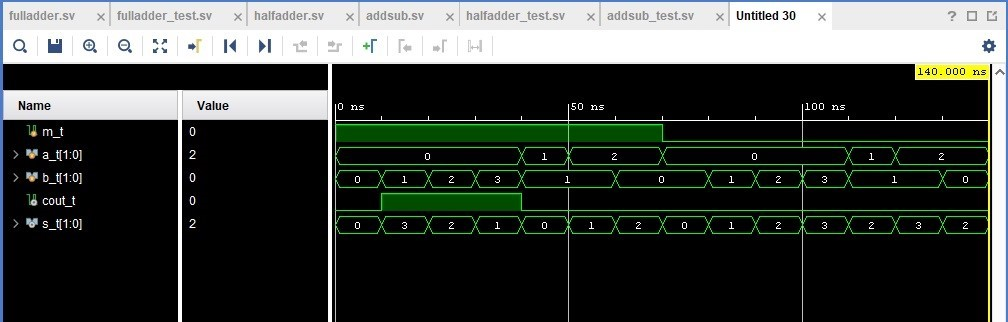
\includegraphics[width=1.0\textwidth]{AddSubReal}
	\caption{2-Bit simulation waveform and ERT}
	\label{fig:sim_with_table}
\end{figure}

\clearpage

The results match what was expected as the screenshotted waveform results confirm the expected results table. 
\section*{Code}
\begin{lstlisting}[style=Verilog,caption=Half Adder Design Code,label=code:ex ]
// Ashlie Lackey and CJ Jones , ELC 2137 , 2020 -2 -13
module halfadder ( input a , b ,
output s , c ) ;
// When using primitive instances , output is always the first port
xor (s , a , b ) ;
and (c , a , b ) ;
endmodule // halfadder

\end{lstlisting}

\begin{lstlisting}[style=Verilog,caption=Half Adder Testbench Code,label=code:ex ]
module example_and(
input a, b,
output c);
// c = a AND b
and(c,a,b);
endmodule
\end{lstlisting}

\begin{lstlisting}[style=Verilog,caption=Full Adder Design Code,label=code:ex ]
// Ashlie Lackey and CJ Jones , ELC 2137 , 2020 -2 -13
module fulladder (
input ain , bin , cin ,
output cout , sout
) ;

// Internal signals
wire c1 , c2 , s1 ;
// One instance of halfadder
halfadder ha0 (
. a ( ain ) , . b ( bin ) ,
. c ( c1 ) , . s ( s1 )
) ;
// second halfadder
halfadder ha1 (
. a ( s1 ) , . b ( cin ) ,
. c ( c2 ) , . s ( sout )
) ;

// Define carry output
xor (cout , c1 , c2 ) ;
endmodule // fulladder

\end{lstlisting}

\begin{lstlisting}[style=Verilog,caption=Full Adder Testbench Code,label=code:ex ]
// Ashlie Lackey and CJ Jones , ELC 2137 , 2020 -2 -13
module fulladder_test () ;
reg cin_t , a_t , b_t ;
wire cout_t , s_t ;
//instantiate fulladder
fulladder FA (. ain ( a_t ) , . bin ( b_t ) , . cin ( cin_t ) , . sout ( s_t ), . cout (cout_t) ) ;
// module here

initial begin
cin_t =0; a_t =0; b_t =0; #10;
//case2
{ a_t , b_t, cin_t } = 3'b100 ; #10;
//case3
{ a_t , b_t, cin_t } = 3'b010 ; #10;
//case4
{ a_t , b_t, cin_t } = 3'b110 ; #10;
//case5
{ a_t , b_t, cin_t } = 3'b001 ; #10;
//case6
{ a_t , b_t, cin_t } = 3'b101 ; #10;
//case7
{ a_t , b_t, cin_t } = 3'b011 ; #10;
//case8
{ a_t , b_t, cin_t } = 3'b111 ; #10;

$finish ;
end

endmodule // fulladder_test

\end{lstlisting}

\begin{lstlisting}[style=Verilog,caption=2-bit Adder Design Code,label=code:ex ]
// Ashlie and CJ , ELC 2137 , 2020 -2 -13
module addsub (
input [1:0] a , b ,
input mode ,
output [1:0] sum ,
output cbout
) ;
// Internal signals
wire c1 , c2 ;
wire [1:0] b_n ;
// Invert b input for subtraction
assign b_n[0] = b[0] ^ mode;
assign b_n[1] = b[1] ^ mode;
//first full adder
fulladder fa0 (
. ain ( a [0]) , . bin ( b_n [0]) , . cin (
mode) ,
. cout ( c1 ) , . sout ( sum [0])
) ;
//second full adder
fulladder fa1 (
. ain ( a [1]) , . bin ( b_n [1]) , . cin (
c1 ) ,
. cout ( c2 ) , . sout ( sum [1])
) ;
// Convert carry to borrow when
// subtracting
assign cbout = c2 ^ mode;
endmodule // addsub

\end{lstlisting}

\begin{lstlisting}[style=Verilog,caption=2-bit Adder Testbench Code,label=code:ex ]
// Ashlie Lackey , ELC 2137 , 2020 -2 -19
module addsub_test () ;
reg m_t;
reg [1:0] a_t, b_t;
wire cout_t ;
wire [1:0] s_t ;
// instantiate adder/subtractor
addsub AS(. a ( a_t ) , . b ( b_t ) , . mode ( m_t ) , . sum ( s_t ), . cbout (cout_t) ) ;
// module here

initial begin
//Subtraction Cases
//case1
{ a_t[1], b_t[1], a_t[0], b_t[0], m_t } = 5'b00001 ; #10;
//case2
{ a_t[1], b_t[1], a_t[0], b_t[0], m_t } = 5'b00011 ; #10;
//case3
{ a_t[1], b_t[1], a_t[0], b_t[0], m_t } = 5'b01001 ; #10;
//case4
{ a_t[1], b_t[1], a_t[0], b_t[0], m_t } = 5'b01011 ; #10;
//case5
{ a_t[1], b_t[1], a_t[0], b_t[0], m_t } = 5'b00111 ; #10;
//case6
{ a_t[1], b_t[1], a_t[0], b_t[0], m_t } = 5'b10011 ; #10;
//case7
{ a_t[1], b_t[1], a_t[0], b_t[0], m_t } = 5'b10001 ; #10;



//Addition Cases
//case8
{ a_t[1], b_t[1], a_t[0], b_t[0], m_t } = 5'b00000 ; #10;
//case9
{ a_t[1], b_t[1], a_t[0], b_t[0], m_t } = 5'b00010 ; #10;
//case10
{ a_t[1], b_t[1], a_t[0], b_t[0], m_t } = 5'b01000 ; #10;
//case11
{ a_t[1], b_t[1], a_t[0], b_t[0], m_t } = 5'b01010 ; #10;
//case12
{ a_t[1], b_t[1], a_t[0], b_t[0], m_t } = 5'b00110 ; #10;
//case13
{ a_t[1], b_t[1], a_t[0], b_t[0], m_t } = 5'b10010 ; #10;
//case14
{ a_t[1], b_t[1], a_t[0], b_t[0], m_t } = 5'b10000 ; #10;

$finish ;
end

endmodule // addsub_test


\end{lstlisting}



\end{document}



\end{document}
